\let\negmedspace\undefined
\let\negthickspace\undefined
\documentclass[journal]{IEEEtran}
\usepackage[a5paper, margin=10mm, onecolumn]{geometry}
%\usepackage{lmodern} % Ensure lmodern is loaded for pdflatex
\usepackage{tfrupee} % Include tfrupee package

\setlength{\headheight}{1cm} % Set the height of the header box
\setlength{\headsep}{0mm}     % Set the distance between the header box and the top of the text

\usepackage{gvv-book}
\usepackage{gvv}
\usepackage{cite}
\usepackage{amsmath,amssymb,amsfonts,amsthm}
\usepackage{algorithmic}
\usepackage{graphicx}
\usepackage{textcomp}
\usepackage{xcolor}
\usepackage{txfonts}
\usepackage{listings}
\usepackage{enumitem}
\usepackage{mathtools}
\usepackage{gensymb}
\usepackage{comment}
\usepackage[breaklinks=true]{hyperref}
\usepackage{tkz-euclide} 
\usepackage{listings}
% \usepackage{gvv}                                        
\def\inputGnumericTable{}                                 
\usepackage[latin1]{inputenc}                                
\usepackage{color}                                            
\usepackage{array}                                            
\usepackage{longtable}                                       
\usepackage{calc}                                             
\usepackage{multirow}                                         
\usepackage{hhline}                                           
\usepackage{ifthen}                                           
\usepackage{lscape}
\usepackage{circuitikz}
\tikzstyle{block} = [rectangle, draw, fill=blue!20, 
    text width=4em, text centered, rounded corners, minimum height=3em]
\tikzstyle{sum} = [draw, fill=blue!10, circle, minimum size=1cm, node distance=1.5cm]
\tikzstyle{input} = [coordinate]
\tikzstyle{output} = [coordinate]


\begin{document}

\bibliographystyle{IEEEtran}
\vspace{3cm}

\title{4.2.2}
\author{AI25BTECH11039-Harichandana Varanasi}
 \maketitle
% \newpage
% \bigskip
{\let\newpage\relax\maketitle}

\renewcommand{\thefigure}{\theenumi}
\renewcommand{\thetable}{\theenumi}
\setlength{\intextsep}{10pt} % Space between text and floats


\numberwithin{equation}{enumi}
\numberwithin{figure}{enumi}
\renewcommand{\thetable}{\theenumi}



\date{}

\begin{document}
\maketitle


\begin{problem}
Find the direction and normal vectors of the line
\begin{align*}                 
    x - \frac{y}{5} - 10 = 10
\end{align*}
\end{problem}



\begin{solution}
\setcounter{equation}{0}
\renewcommand{\theequation}{\arabic{equation}}
Find the direction and normal vectors of the line
\begin{align}
    x - \frac{y}{5} - 10 &= 10
    \label{eq1}
\end{align}

Rewriting \eqref{eq1},
\begin{align}
    x - \frac{y}{5} &= 20
    \label{eq2}
\end{align}

Comparing with the standard form
\begin{align}
    \vec{n}^T\vec{x} &= c,
    \label{eq3}
\end{align}
we obtain
\begin{align}
    \vec{n} = \myvec{1 \\ -\tfrac{1}{5}}, \quad
    \vec{x} = \myvec{x \\ y}, \quad
    c = 20
    \label{eq4}
\end{align}

Thus, the normal vector is
\begin{align}
    \vec{n} = \myvec{1 \\ -\tfrac{1}{5}}
    \label{eq5}
\end{align}

From the orthogonality condition,
\begin{align}
    \vec{m}^T\vec{n} = 0
    \label{eq6}
\end{align}

Let
\begin{align}
    \vec{m} = \myvec{1 \\ 5}
    \label{eq7}
\end{align}
which satisfies \eqref{eq6}.

Hence, the required vectors are
\begin{align}
    \text{Direction vector: } \vec{m} = \myvec{1 \\ 5} \label{eq8}\\
    \text{Normal vector: } \vec{n} = \myvec{1 \\ -\tfrac{1}{5}} \label{eq9}
\end{align}
\end{solution}




     \begin{figure}[h!]
\centering
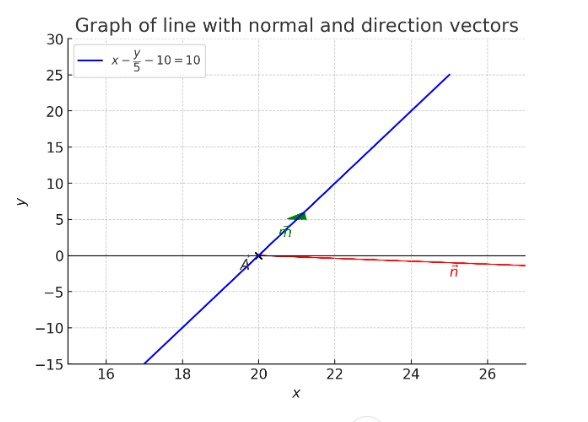
\includegraphics[width=0.5\linewidth]{figs/matgeo 4.2.2.jpeg}
 \caption{Line $x - \tfrac{y}{5} - 10 = 10$ with direction $\vec{m}$ and normal $\vec{n}$.}
    \label{fig:4.2.2}


\end{figure}

\end{document}
